\chapter{System-wide Design Decisions}

In this chapter, the decision for the system-wide detailed design is made.

\section{Input and Output}
The system shall get inputs from the various users, from sensors on the Dismounted COP and from external databases. The inputs from the user is registered either in the HQ or on the Dismounted COP. The external databases gives input to the Server, which distributes the data to the HQ and the Dismounted COP. The system gives outputs from the Server, the HQ and the Dismounted COP.

A description of the various users, is given in the System Requirements Specification section 2.1.

\section{Behavior Resulting from I/O}
The Server shall receive and distribute data in the system according to the modes the users
are using. The Server also distributes system updates. The Dismounted COP shall give
warnings if the sensors register a dangerous value. Both the HQ and the Dismounted COP
shall show the information selected by the user, according to the selected mode. When
an audio command is given from the the HQ, the Dismounted COP must play the audio
command to the user. The HQ controls the connection to the Dismounted COP, meaning
that the HQ chooses which Dismounted COP it will be connected to.

\section{User interaction with system}

The system consists of two overall devices: A COP for the mobile HQ and a dismounted COP. The user interface to the two devices are somewhat similar, and is described the following paragraphs. 

\paragraph{COP}
\begin{enumerate}
\item[•] \textbf{Touchscreen:} \\
The primary interface of the dismounted COP is the touchscreen of the device. The touchscreen lets the user navigate in the application through touch inputs. 

\item[•] \textbf{Microphone:} \\
The microphone is part of the audio user interface. It allows the user to navigate in the application through voice commands. Furthermore, it is part of a telecommunication interface between the SitaWare Civilian users. 

\item[•] \textbf{Speaker:} \\
The speaker is part of the audio user interface. It provides the user with warning sounds in case of dangerous radiation, temperatur or oxygen levels. Furthermore, it is part of a telecommunication interface between the SitaWare Civilian users.

\item[•] \textbf{Keyboard:}\\
The keyboard is an optional interface to the COP that accompanies the touchscreen in letting the user navigate in the application. The keyboard is used by the user to navigate in the application through touch inputs. 

\item[•] \textbf{Mouse:}\\
The mouse is an optional interface to the COP that accompanies the touchscreen in letting the user navigate in the application. The mouse is used by the user to navigate in the application through touch and movement inputs. 
\end{enumerate}


\paragraph{Dismounted COP}

\begin{enumerate}
\item[•] \textbf{Touchscreen:} \\
The primary interface of the dismounted COP is the touchscreen of the device. The touchscreen lets the user navigate in the application through touch inputs. 

\item[•] \textbf{Microphone:} \\
The microphone is part of the audio user interface. It allows the user to navigate in the application through voice commands. Furthermore, it is part of a telecommunication interface between the SitaWare Civilian users. 

\item[•] \textbf{Speaker:} \\
The speaker is part of the audio user interface. It provides the user with warning sounds in case of dangerous radiation, temperatur or oxygen levels. Furthermore, it is part of a telecommunication interface between the SitaWare Civilian users.
\end{enumerate}

\section{Safety, Security, and Privacy}
The system has 3 modes to ensure the correct user rights. The default mode is for normal actors in the field. The Commander mode is for the commanding users. The Administrator mode is for service personal, for maintaining purposes. All data must be encrypted. 

\section{Physical Aspects}
\begin{figure}[H]
\centering
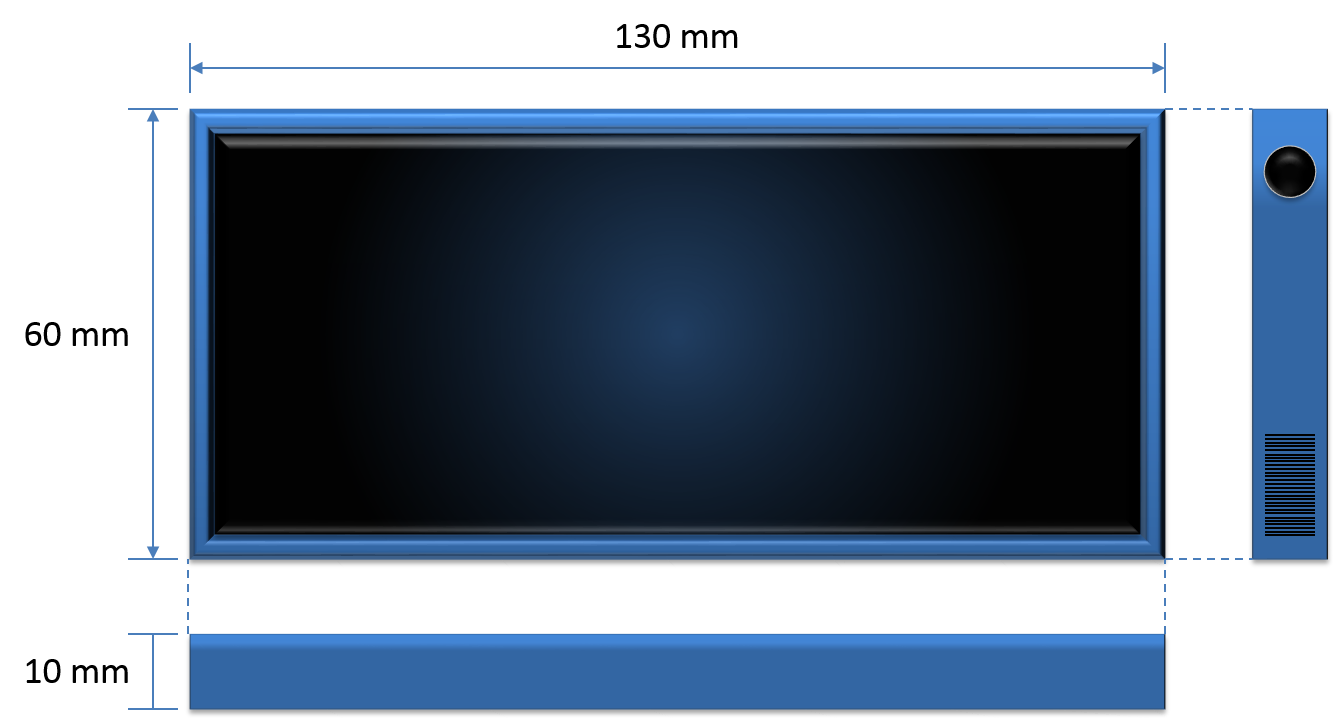
\includegraphics[width=0.95\textwidth]
{Billeder/PhysicalAppearence.png}
\caption{Physical appearence of the Dismounted device.}
\label{fig:PhysicalAppearence}
\end{figure}

\section{Appearance of GUI}
\fixme{Indsæt GUI mock-ups}

%\section{Parts Decisions}
%\textbf{The HQ} shall be a stationary post mounted in a mobile vehicle. The COP shall be implemented on a PC. The user interaction is supposed to be a mix between use of mouse, keyboard and touch screen. It must be possible to give all commands from here. The PC must have a wireless internet connection. To process data the PC must have a processor.\\
%
%\textbf{The Dismounted COP} shall be mounted on the wrist of the user. Therefor the Dismounted COP must be within dimensions of 13x6x1 cm. It must be shock-, water- and heat resistant. The Dismounted COP must have a touch screen which can be used with or without gloves. Furthermore the Dismounted COP must be able to alert the users about radiation, low oxygen levels and dangerous temperatures.\\
%
%\textbf{A Server} shall be used to distribute data between users. It must contain a database for storage of relevant information. The server must also be able to communicate with other SitaWare solutions.\\
%
%For reference purposes the decisions are listed below:
%\begin{description}
%\item[SDD-0100] The COP shall be implemented on a PC.
%\item[SDD-0110] The PC shall have a Touch screen, to display relevant information and to make user interaction easy.
%\item[SDD-0120] The PC shall have a mouse, to make user interaction easy.
%\item[SDD-0130] The PC shall have a keyboard, to make user interaction easy.
%\item[SDD-0140] The PC shall have a GPS, to get the location of the HQ.
%\item[SDD-0150] The PC shall have a Telecommunication module, to access the internet.
%\item[SDD-0160] The PC shall have a speaker, to enable audio communication.
%\item[SDD-0170] The PC shall have a microphone, to enable audio communication.
%\item[SDD-0180] The PC shall have a processor, to process data.
%\item[SDD-0200] The system shall have a Dismounted COP.
%\item[SDD-0210] The Dismounted COP shall have a GPS, to get the location of the Dismounted COP.
%\item[SDD-0220] The Dismounted COP shall have a Micro Controller, to process data.
%\item[SDD-0230] The Dismounted COP shall have a Telecommunication module, to access the internet.
%\item[SDD-0240] The Dismounted COP shall have a Touch screen, to display relevant information and to make user interaction easy.
%\item[SDD-0250] The Dismounted COP shall have a speaker, to enable audio communication.
%\item[SDD-0260] The Dismounted COP shall have a microphone, to enable audio communication.
%\item[SDD-0270] The Dismounted COP shall have a battery, to be mobile.
%\item[SDD-0280] The Dismounted COP shall have a Radiation sensor to alert the user about radiation.
%\item[SDD-0290] The Dismounted COP shall have an Oxygen sensor to alert the user about low oxygen levels.
%\item[SDD-0299] The Dismounted COP shall have a Temperature sensor to alert the user about dangerous temperatures.
%\item[SDD-0300] The system shall have a Server to distribute data.
%\item[SDD-0310] The Server shall have a Database to store information.
%\end{description}

